

\section*{Einleitung}
Diese Arbeit beschäftigt sich mit der Layout-Segmentierung von Digtalisierten Dokumenten mittels Neuronaler Netzwerke.

\cref{chap:documents} beschreibt die Motivation für die Dokumentensegmetierung und aktuelle Entwicklungen im
Bereich der Dokumenten-Digitalisierung.

\cref{chap:reproduktion} nähert sich dem aktuellen Forschungsstand mittels der Reproduktion von zwei Forschungsergebnissen.

\cref{chap:selfsupervised} erläuter die Methode des selbstüberwachten Lernen. Die Methode wird auf die reproduzierten Forschungen angewendet.

%-------------------------------------------------------------------------------
\chapter{Digitalisierte Dokumente}
\label{chap:documents}
% Warum scannt man Dokumente

% Was für Dokumente werden gescannt

% 
Schon in den 50er Jahren begann die Forschung im Bereich der Optischen Zeichenerkennung 
(engl. OCR)\autocite{DoermannHandbookdocumentimage2014}. OCR fand zuerst Einsatz in genau 
spezifizierten Problembereichen zum Beispiel die Erkennung von Druckbuchstaben einer Schreibmaschine. 
Je mehr Dokumente digitalisiert wurden, desto klarer wurde es das Dokumente mehr als 
eine Kette von Zeichen sind. 
Information können in Dokumenten über die Position der Zeichen und Skalierung von Zeichen vermittelt werden.
Zum anderen bestehen Dokumente aus Inhalten die semantische Bedeutung haben, aber nicht als Zeichenkette codiert werden können. 
Eine Randnotiz\marginnote{Der Bezug dieses Satzes zum Text wird durch die Position verdeutlicht} setzt sich durch Formatierung und Position vom restlichen Text ab. 

Wirtschaftsinteressen trieben die Entwicklungen von Dokumentenverarbeitungssystemen in einigen Bereichen sehr weit voran, wie 
zum Beipspiel bei der Verarbeitung von Geschäftsbriefen und Formularauswertung.
Eine Spezialisierung auf bestimmte Dokumentenklassen ist immer noch eine notwendigkeit angesichts der unzähligen, veränderbaren und nicht fest gelegten Gestaltungsmöglichkeiten für Dokumente \parencite[69]{BairdEvolutionDocumentImage2014}.


\section{Digitale Bibliotheken}
\cite{BairdDigitallibrariesdocument2003}

\section{Schritte in der Verarbeitung von Dokumentenbildern}
Die Dokumentensegmetierung ist ein Vorverarbeitungsschritt für weitere Schritte der Dokumentenverarbeitung.

Im Bereich der Bibliotheswissenschaften besteht ein großes Interesse an Klassifizierung von
Buchseiten zur besseren Erschließung.
\cite{McConnaugheyLabeledSegmentationPrinted2017} klassifizieren Buchseiten anhand von textbasierten Features in 4 Kategorien. 
Flow

\section{Auswahl und Beschreibung der Datensätze}
\textcite[985\psqq]{DoermannHandbookdocumentimage2014} listen 5 Aspekte die bei der Erstellung von Datensätzen zu beachten sind:
Auswahl der Daten
Datenbeschaffung
Ground Truth Definition
Ground Trouth Annotation
Speicherformat
Struktur und Organisation

\section{DIVA-HisDB}
Die DIVA \marginnote{\url{http://diuf.unifr.ch/main/diva/}}(Document, Image and Voice Analysis) Gruppe der Universität Fribourg hat im Kontext der Forschungsprojekte HisDoc und HisDoc 2.0 
das Datenset DIVA-HisDB. erstellt.
Die HisDoc-Projekte beschäftigen sich mit der automatischen Analyse von historischen Dokumenten und
wie man diese für Historiker nutzbar machen kann.

Für den Datensatz wurden Dokumente mit komplexen Layout aus der Virtuellen Manuskriptbibliothek der Schweiz (\url{http://www.e-codices.unifr.ch/en}) ausgesucht. Die Manuskripte enthalten neben dem Haupttext auch Randnotizen und Text-Dekorationen. Randnotizen befinden sich auch teilweise zwischen den Zeilen des Haupttexts.
 
DIVA-HisDB besteht aus 150 Dokumenten, aufgeteilt in Trainings-, Validierungs- und Testset (siehe \cref{table:hisdb_pages}. Hinzu kommen 30 Seiten die 
für die finale Wertung des Wettbewerbs ``ICDAR2017 Competition on Layout Analysis for Challenging Medieval Manuscripts'' verwendet wurden.

\begin{table}
    \caption{Aufteilung der Seiten des DIVA-HisDB-Datenssets}
    \label{table:hisdb_pages}
    \begin{tabular}{lccccc}
        {\bfseries Name} & {\bfseries Auflösung} & {\bfseries Training} & {\bfseries Validierung} & {\bfseries Test} & {\bfseries Test ICDAR 2017)}\\
        \csvreader[head to column names]{tables/diva_hisdb_specs.csv}{}%
        {\name&	\width \(\times\)\height & \train	&\validate	&\test	&\comp\\}
    \end{tabular}
\end{table}

Die Manuskripte wurden mit einer Auflösung von 600 dpi gescannt und sind im  JPEG-Format gespeichert. Die \cref{table:hisdbsamples} zeigt Beispiele aus den drei Datensätzen. 



Der Datensatz wurde semi-automatisch mit 3 Annotation (Haupttext, Kommentare, Dekorationen) versehen.
Diese Ground-Truth-Annotationen sind im PAGE-XML-Format und als ``pixel-label'' PNG-Bilder gespeichert.
Die Menge an Pixeln pro Klasse ist sehr unterschiedlich.
Die \cref{table:class_distribution} zeigt das in jedem Dokumentenset der Hintergrund deutlich überwiegt.

\begin{table}
    \caption{Verteilung der Klassen in Prozent\autocite[1362]{SimistiraICDAR2017CompetitionLayout2017}}
    \label{table:class_distribution}
    \begin{tabular}{lrrrr}
        {\bfseries Set} & {\bfseries Hintergrund} & {\bfseries Kommentar} & {\bfseries Dekoration} & {\bfseries Text}\\
        \csvreader[head to column names]{tables/diva_hisdb_class_distribution.csv}{}%
        {\set&	\background & \comments & \decoration & \text \\}
    \end{tabular}
\end{table}


\begin{table*}
    \begin{tabular}{llp{4cm}}
        \vspace{0.2cm}
        {\bfseries Seite} & {\bfseries Detailauschnitt} & {\bfseries Quelle } \\
        \vspace{0.5cm}
        
        \raisebox{-.5\height}{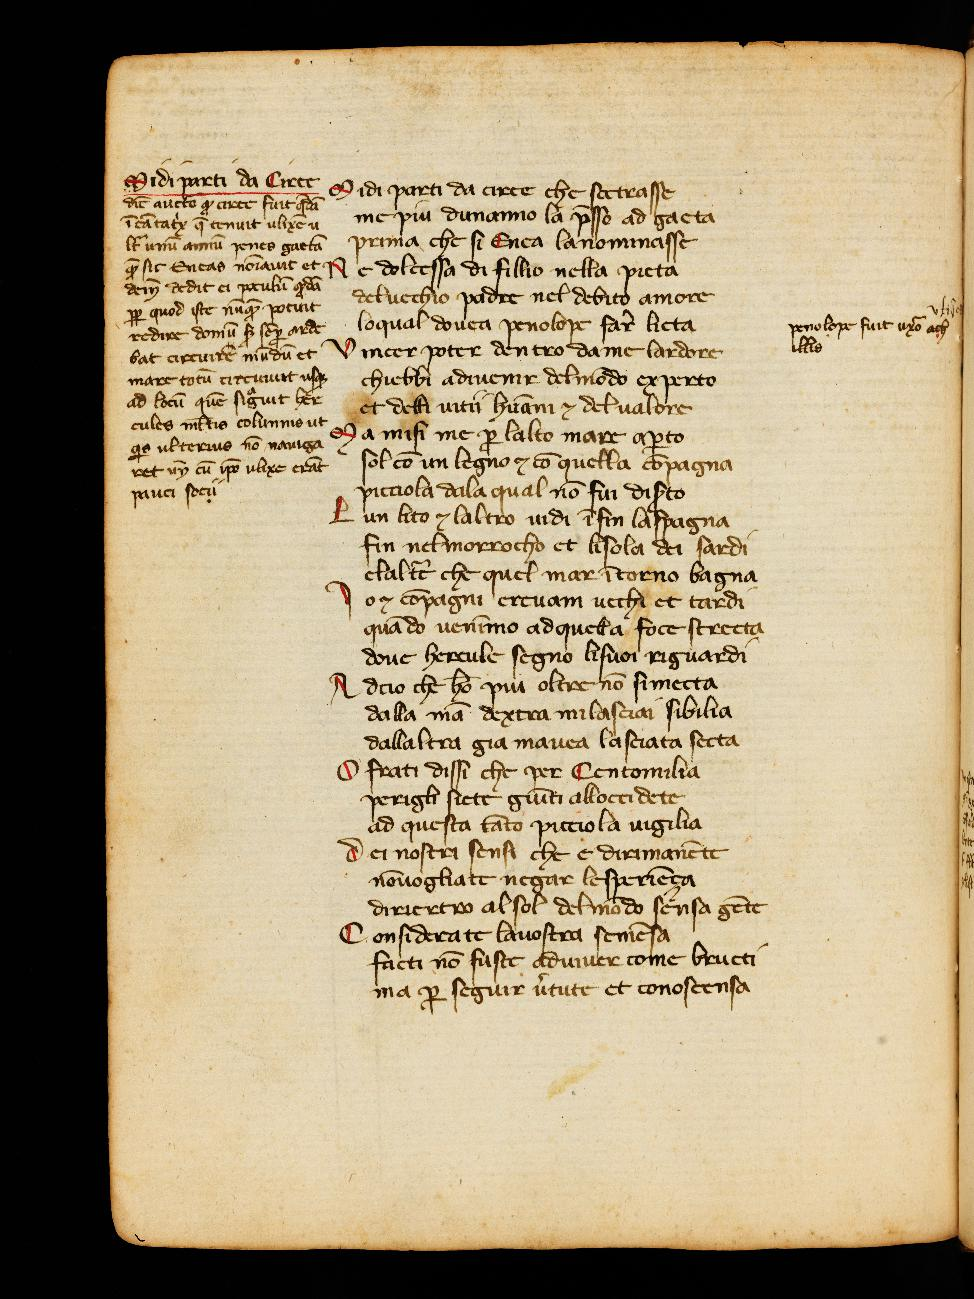
\includegraphics[height=4cm]{figures/datasets/HisDBSample0.jpeg}}
    &\raisebox{-.5\height}{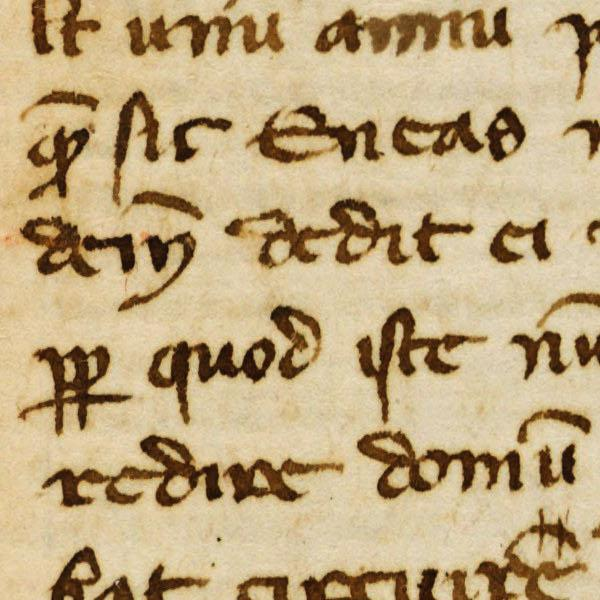
\includegraphics[height=4cm]{figures/datasets/HisDBSampleBox0.jpeg}}
     & \citefield{AlighieriColognyFondationMartin1300}{title}\\
     \vspace{0.5cm}  
     
    \raisebox{-.5\height}{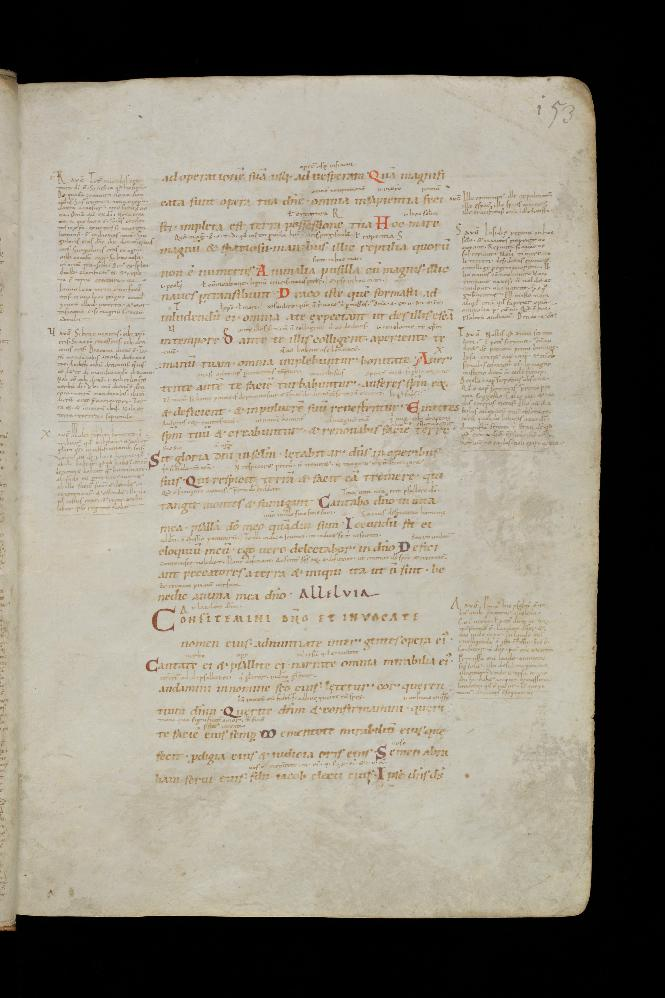
\includegraphics[height=4cm]{figures/datasets/HisDBSample2.jpeg}}
    & \raisebox{-.5\height}{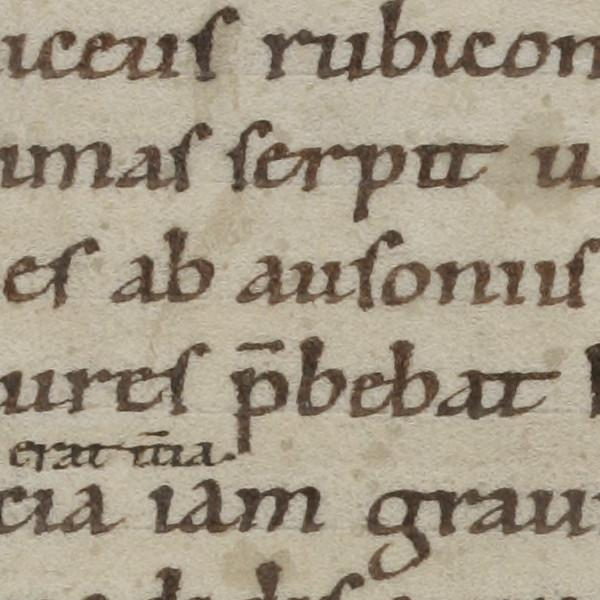
\includegraphics[height=4cm]{figures/datasets/HisDBSampleBox2.jpeg}}
    & \citefield{AmbrosiusStGallenStiftsbibliothek985}{title}\\
    \vspace{0.5cm}
    
     \raisebox{-.5\height}{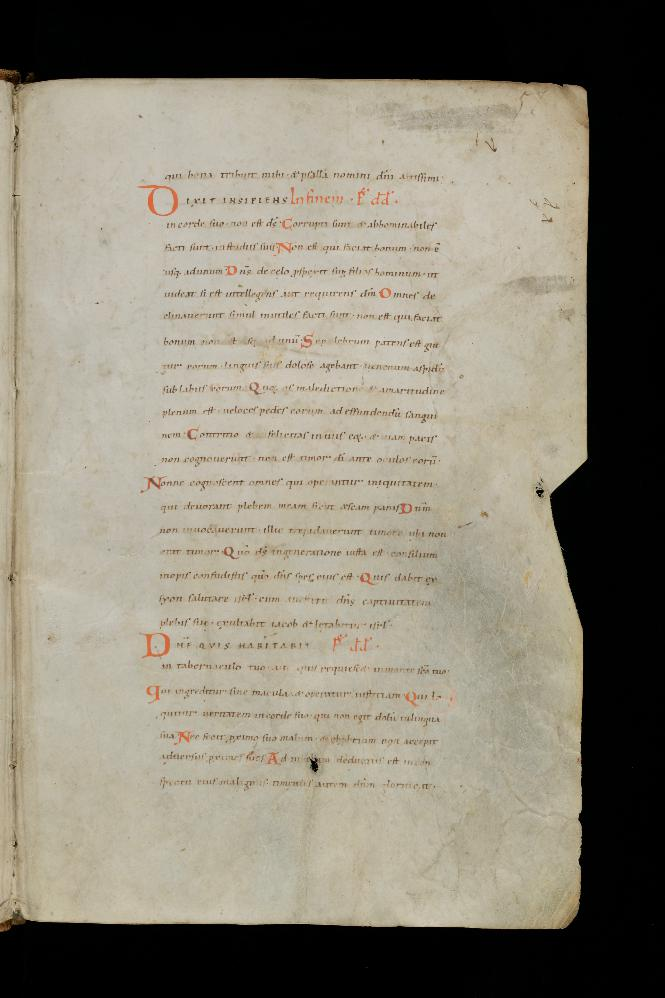
\includegraphics[height=4cm]{figures/datasets/HisDBSample1.jpeg}}
    &\raisebox{-.5\height}{
\includegraphics[height=4cm]{figures/datasets/HisDBSampleBox1.jpeg}}
     & \citefield{LucanusStGallenStiftsbibliothek1025}{title}\\
     \vspace{0.5cm} 

    \end{tabular}
    \caption{HisDB Beipsiele mit Detailauschnitt}
    \label{table:hisdbsamples}
\end{table*}


%-------------------------------------------------------------------------------
\chapter{Reproduktion bisheriger Ergebnisse}
\label{chap:reproduktion}
\epigraph{What I cannot create, I do not understand}{--- Richard Feyman}

\qq{Warum NN?}
Künstliche Neuronale Netzwerke (kurz NN) dominieren den Forschungsbereich der 
Bilderkennung. 
Besonders die Klasse der faltenden Neuronalen Netzwerks \engl{convolutional neural network}, kurz CNN, konnte viele Erfolge für sich beanspruchen.
Rekordbrechende Ergebnisse bei der Klassifiziererung von handgeschriebenen Ziffern \parencite{LeCunBackpropagationappliedhandwritten1989} und des ImageNet-Wettbewerbs \parencite{KrizhevskyImageNetClassificationDeep2012a} motivieren dazu CNN-Methoden auch in anderen
Bereichen anzuwenden.

\begin{marginfigure}
    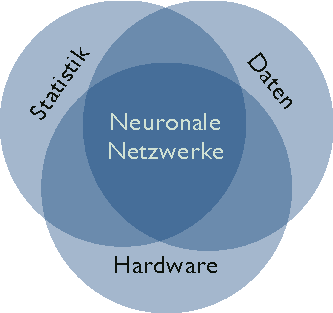
\includegraphics[width=\textwidth]{figures/tasks/nn_areas_venn.pdf}
    \caption{Diziplinen im Bereich Neurale Netzwerke}
    \label{fig:chen:cnn_task}
\end{marginfigure}
Neurale Netzwerke benötigen weniger Entwicklungsaufwand und können zudem einfacher von 
 wachsenden Rechenkapazitäten und Datenmengen gebrauch machen \parencite[436]{LeCunDeeplearning2015}. 
Aber die Wissenschaft der NN ist ein Feld, dass durch die aktuelle Praxis mehr als durch Theorie geprägt ist. 
Das bedeuted zum einen das theoretische Grundlagen noch nicht gefestigt sind.
Zum anderen ist die Theorie nur eine Faktor für den erfolgreichen Einsatz von NNs. 
Je mehr Parameter unklar sind desto schwieriger wird eine Reproduktion.
\qq{Unterschied replikation, reproduktion?}
Die Reproduktion von Ergebnissen ist aber ein wichtiger Bestandteil in jedem Forschungsgebiet. 

\qq{welche Experimente?}
Im folgenden werden Paper genauer untersucht, die sich mit dem Problem der Dokumentensegmentierung mit Hilfe von CNNs nähern.
Das erste Experiment basiert auf dem neusten Paper von Mitgliedern der DIVA-Gruppe: \citeauthor*{ChenConvolutionalNeuralNetworks2017}. 

Das zweite Experiment basiert auf der Forschung des Gewinners des IDCAR2017-Wettbewerbs: \citeauthor*{XuPageSegmentationHistorical2017} 

\section{Andere Ansätze}
\cite{WickFullyConvolutionalNeural2017}


\section{Bildverarbeitung mittels Neuronaler Netzwerke}
Neurale Netwerke und CNN sind Beispiele für Machinenlernalgorithmen \engl{maschine learning algorithm}.
\cite{MitchellMachinelearning1997} definiert einen Machinenlernalgorithmus wie folgt: ``A computer program is said to learn from experience E with respect to some class of tasks T and perfomance measure P, if its performance at tasks T, as measured by P improves with experience E''.

Für die meisten Anwendungen ist die Aufgabe T eine Klassifizierungsaufgabe.
Der Lernalgorithmus soll eine Funktion \(f: \mathds{R}^n \Leftarrow \left\{1,\dots,k \right\} \) so das \(y = f\left(x\right)\) \cite[97]{GoodfellowDeeplearning2016}.


\cite[393]{Hastieelementsstatisticallearning2009}: linear Kombinationen der Eingabe as Features. Target als nonlineare Funktion dieser Features modelieren.  
\begin{marginfigure}
    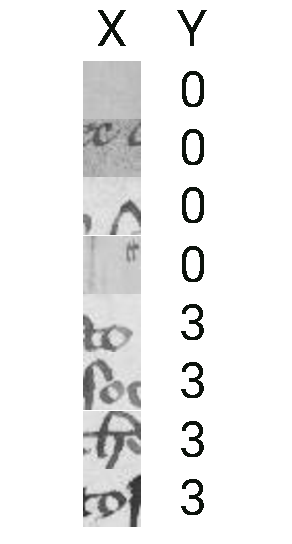
\includegraphics[width=\textwidth]{figures/tasks/chen_examples.pdf}
    \caption{TODO}
    \label{fig:chen:cnn_task}
\end{marginfigure}
\section{SGD}
\section{Aktivierungsfunktionen}
\subsection{ReLU}
\begin{align}
    f\left(x\right) &= \text{max}(0,x)
\end{align}
\subsection{Softmax}


\section{CNN}
\qq{Filter als vorläufer von CNN}
CNN kombinieren zwei Konzepte der Bilderverarbeitung: Neuronale Netzwerke und Filter.
Klassifikationsprobleme wurde traditionell in zwei Schritten gelöst. Zuerst wurden 
Featuredeskriptoren entwickelt welche dann als Input für trainierbare Klassifizierer 
verwendet wurden \autocite[2353]{RawatDeepConvolutionalNeural2017}.

\qq{Filterbeispiel?}
\qq{}

\section{\textcite{ChenConvolutionalNeuralNetworks2017}}
Das Paper ``\citetitle*{ChenConvolutionalNeuralNetworks2017}'' von \citeauthor*{ChenConvolutionalNeuralNetworks2017} betrachten die Dokumentensegmentierung 
als ``pixel labeling problem''. Einem Pixel wird eine Klasse zugewiesen indem
ein CNN die Umgebung des Pixels analisiert. 
Jedoch ist eines der größten Probleme bei der Verarbeitung von Dokumentenseiten die Größe.
Die Bilder im HisDB-Datenset sind mit einer Auflösung von \(4872 \times 6496\) wesentlich größer als andere Datensets.\qq{Welche?}
Um den Prozess zu beschleunigen werden nicht alle Pixel sondern nur etwa 3000 Pixelcluster klassifiziert. 

\subsection{Vorverarbeitung}
\citeauthor{ChenConvolutionalNeuralNetworks2017} skalieren alle Bilder mit einem Faktor von  \(2^{-3}\) und wenden dann den Superpixelalgorithmus SLIC (simple linerar iterative clustering) an \parencite{AchantaSLICSuperpixels2010} um die Dokumentenseiten in Superpixel einzuteilen.
Ein \(28 \times 28\)-Bereich um das Zentrum des Superpixel wird dann mithilfe eines CNN
klassifiziert. Diese Klassifizierung wird dann allen Pixel innerhalb des Superpixels zugewiesen.

\section{SLIC Superpixel}
Der SLIC-Algorithmus basiert auf dem k-Means-Algorithmus und teilt Pixel inhalb eines 5D-Raums in Cluster ein. 
In jedem Arbeitsschritt werden Pixel dem Clusterzentrum mit der geringsten Distanz zugeordnet und danach werden die Clusterzentren neu berechnet.
Das Distanzmaß \(D_s\) zu den Clusterzentren \(k=[1,K]\) basiert auf den Farbabstand im Lab-Farbraum \(d_{lab}\) und den räumlichen Abstand \(d_{xy}\):

\begin{align}
    d_{lab} &= \sqrt{ \left( l_k - l_i \right)^2 + \left( a_k - a_i \right)^2 + \left( b_k - b_i \right)^2 }\\
    d_{xy}  &= \sqrt{ \left( x_k - x_i \right)^2 + \left(y_k - y_i \right)^2 }\\
    D_{s}   &= d_{lab} + \frac{m}{S} d_{xy}
\end{align}

Der Faktor \(m\) ermöglicht eine Gewichtung den zwei Distanzmaßen. Je höher
der Faktor desto kompakter werden die Superpixel. \cref{fig:slic_parameters}
zeigt das Ergebniss des Algorithmus mit unterschiedlichen Parameter  \(m\)
angewendet auf eine Dokumentenseite.

\begin{figure}
    \centering
    \caption{Die SLIC-Pixelgrenzen sind in rot dargestellt }
    \label{fig:slic_parameters}
    \subfloat[ \(m = 0.1\)]{
        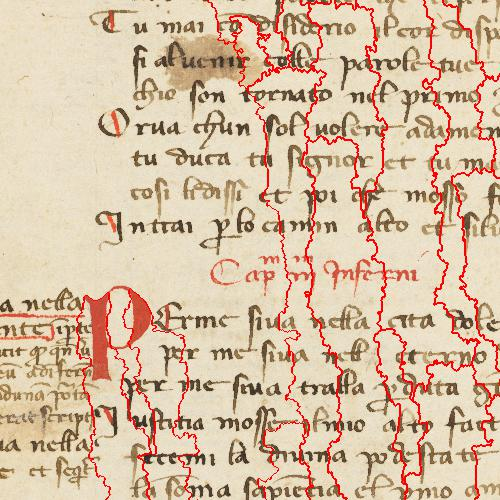
\includegraphics[width=0.24\textwidth]{figures/img/mark_boundaries_m0.jpg}
    }
    \subfloat[\(m = 1\)]{
        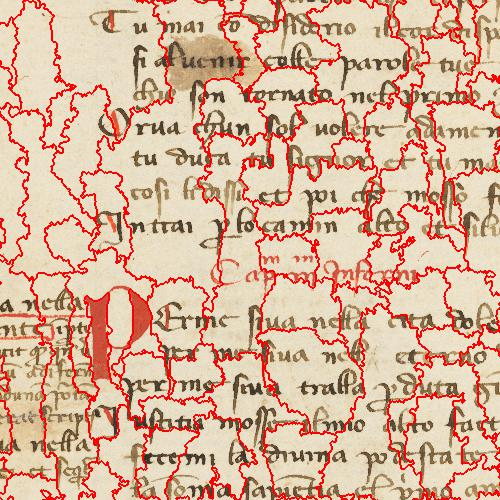
\includegraphics[width=0.24\textwidth]{figures/img/mark_boundaries_m1.jpg}
    }
    \subfloat[\(m = 10\)]{
        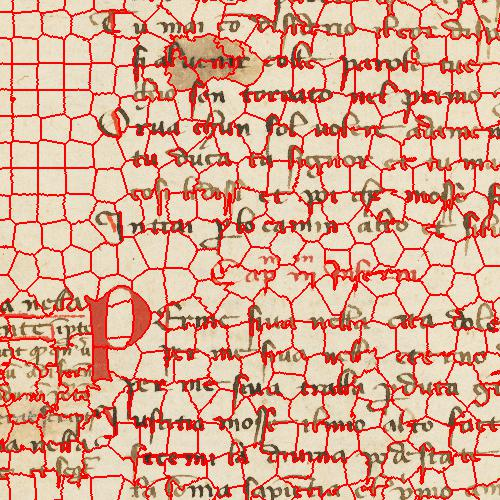
\includegraphics[width=0.24\textwidth]{figures/img/mark_boundaries_m10.jpg}
    }
    \subfloat[\(m = 100\)]{
        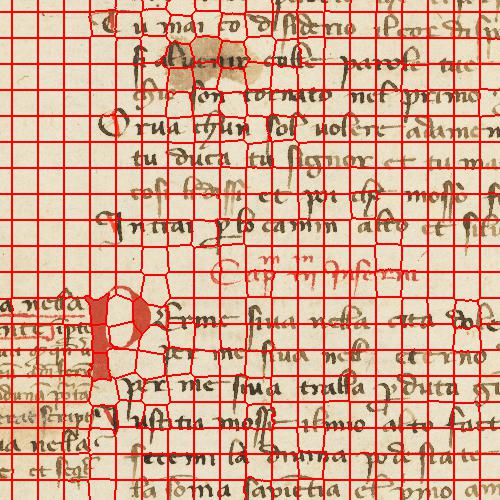
\includegraphics[width=0.24\textwidth]{figures/img/mark_boundaries_m100.jpg}
    }
\end{figure}

\citeauthor{AchantaSLICSuperpixelsCompared2012} stellen später zwei wichtige Erweiterungen vor:
Normalisierung des Distanzmaßes und Adaptive-SLIC.

\citeauthor{ChenConvolutionalNeuralNetworks2017a} nennen keine Details zur Wahl
der Superpixel-Parameter, nennen aber eine frühere Studie die sich mit unterschiedlichen 
Superpixel verfahren beschäftigt \parencite{ChenPageSegmentationHistorical2016}.
Die Studie versucht einen Autoencoder (siehe \ref{sec:autoencoder}) zu trainieren auf Basis von Superpixeln und vergleicht dabei den Einfluss von unterschiedlichen Superpixel-Methoden. Die veröffenlichen Ergebniss zeigen aber nur die Performanz im Bezug
auf die Zahl der Cluster \(n \in \left\{10^3, 50^3, 100^3, 200^3\right\}\) und dem Skalierungsfaktor \(\alpha \in \left\{2^{-2}, 2^{-3}\right\}\)
\qq{adaptive slic}
\qq{Problem gt zu treffen}

\section{CNN-Architektur}
\citeauthor{ChenConvolutionalNeuralNetworks2017a} beschreiben die Struktur
des CNN als \(28 \times 28 \times 1 - 26 \times 26 \times 4 - 100 - M\).

Während des Trainings wird das Ground-truth Label des Zentrumpixels als Label für den Superpixel verwendet.


\section{Xavier initialization}


\section{Dropout}



\section{Training}


\section{\textcite{XuPageSegmentationHistorical2017}}
Das Paper \citetitle*{XuPageSegmentationHistorical2017} von \citeauthor*{XuPageSegmentationHistorical2017} verfolgt einen anderen Ansatz.
\citeauthor{XuPageSegmentationHistorical2017} verwenden eine Netwerk  


\section{VGG}
\section{Deconvolution}
\section{Ergebnisse}
%-------------------------------------------------------------------------------
\chapter{Selbstüberwachtes Lernen}
\label{chap:selfsupervised}
\qq{Warum besteht interesse an unsupervised/selfsupervised Lernen?}
Ein Teil des Erfolges von CNNs ist auf die Verfügbarkeit von großen annotierten Datensätzen wie ImageNet zurückzuführen
\autocite{SunRevisitingUnreasonableEffectiveness2017}.
Jedoch ist die Anzahl der Bilder im ImageNet-Datensatz in den vergangen Jahren gleich geblieben, während die  verfügbare Netzwerkkapazität und GPU-Rechenleistung angestiegen ist.
\citeauthor{SunRevisitingUnreasonableEffectiveness2017} zeigen mithilfe des JFT-300M-Datensets (300 Millionen annotierte Bilder), dass die Performanz von allen getesteten Aufgaben (Klassifizerung, Segmentierung, etc.)
logaritmisch zur Datenmenge ansteigt. 

Für einen linearen Performanzanstieg bräuchte man exponetiell mehr Daten.
Die Annotierung von Datensets ist immer ein teuerer Prozess \autocite[988]{ValvenyDatasetsAnnotationsDocument2014}.
Die manuelle Annotation einer Dokumentenseite kann mehr als eine Stunde in Anspruch nehmen. 

% Das kollaborative Annotieren von Datensets ermöglicht es große Datenmengen in hoher Qualität zu annotieren.
% Das reCAPTCHA-Projekt \cite{reCAPTCHA} h  
% semiautomatisch



\begin{figure}[htbp!]
    \centering
    \caption{Schematische Darstellung von ML-Methoden}
    \label{fig:ml_methods}
    \subfloat[Neuronales Netzwerke und Training \cite{CholletDeeplearningPython2018}\label{fig:sub1}]{    
      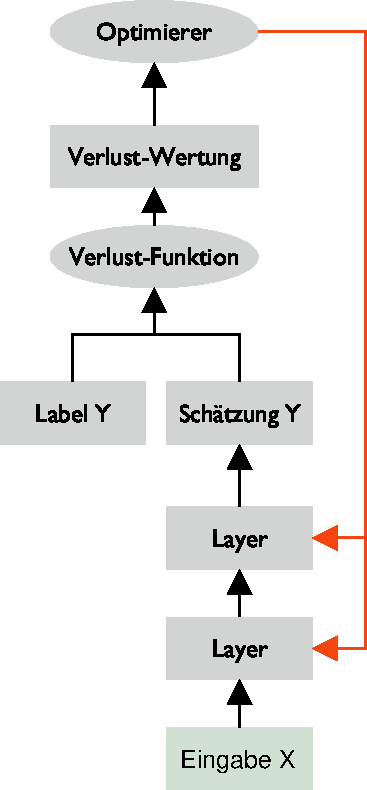
\includegraphics[width=0.3\textwidth, valign=t]{figures/graphs/chollet2018supervised.pdf}
      \vphantom{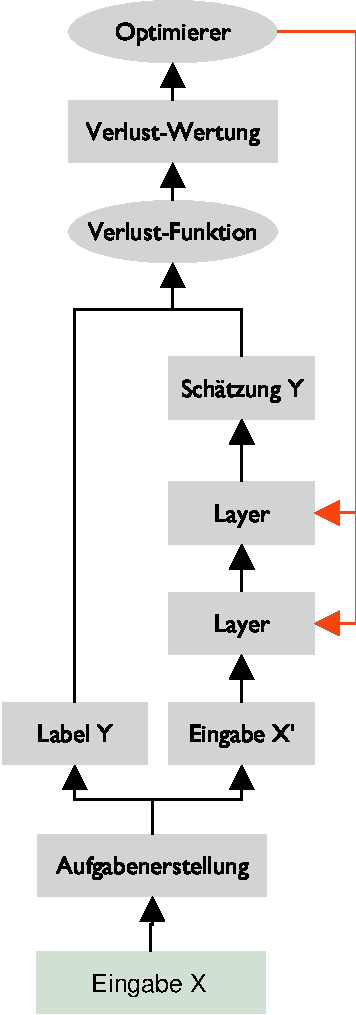
\includegraphics[width=0.3\textwidth,valign=t]{figures/graphs/selfsupervised.pdf}}
    }
    \subfloat[Autoencoder\label{fig:sub2}]{    
      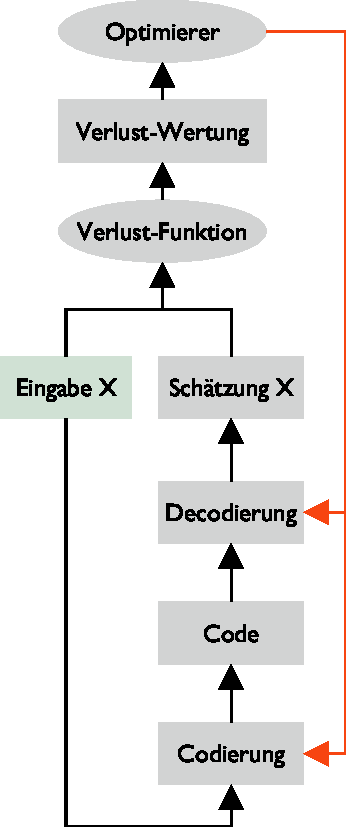
\includegraphics[width=0.3\textwidth, valign=t]{figures/graphs/autoencoder.pdf}
      \vphantom{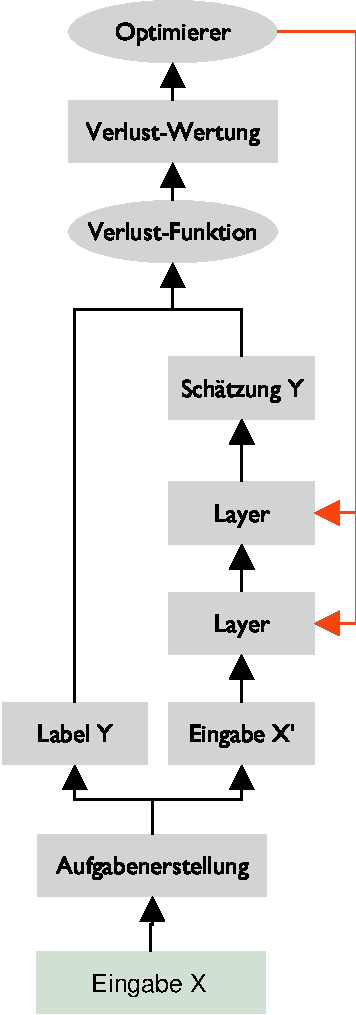
\includegraphics[width=0.3\textwidth,valign=t]{figures/graphs/selfsupervised.pdf}}
    }
    \subfloat[Selbstüberwachtes Lernen\label{fig:sub3}]{    
      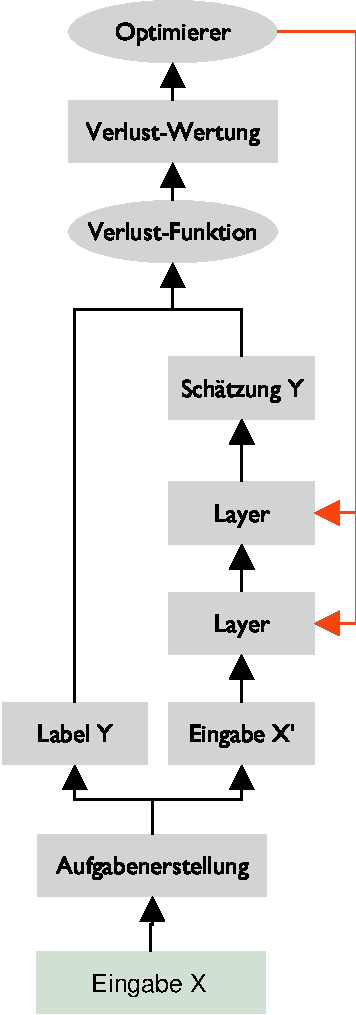
\includegraphics[width=0.3\textwidth, valign=t]{figures/graphs/selfsupervised.pdf}
    }
    
    
\end{figure}
\vspace{0.5cm}



\section{Unüberwachtes Lernen von unterscheidbaren Features}

\sfigure{Workflow}{figures/graphs/dosovitskiy2015_workflow.pdf}

Jigsaw
\cite{NorooziUnsupervisedLearningVisual2016}
% \begin{figure}
%     \includegraphics[]{figures/graphs/exp.pdf} 
%     \caption{Image}
%   \end{figure}

\cite{DosovitskiyDiscriminativeUnsupervisedFeature2016} Loss-Funktion skaliert nicht auf viele Klassen.
Letzter Klassifiezierungslayer ist Fully-Connected. Je mehr Image-Patches desto mehr Parameter.

\cite{DoerschMultitaskSelfSupervisedVisual2017} benutzt Triplet-Loss.
Der Verlust wird mit einem Positiv und einem Negativbeispiel berechnet.
Die Idee dafür kommt von \citeauthor{WangUnsupervisedLearningVisual2015}.
Die Kosinus-Ähnlichkeit misst den Winkel zwischen zwei Vektoren. Vektoren mit einem Winkel von 0 haben
eine Kosinus-Maß von 1. Der größtmögliche Winkel hat eine Kosinusmaß von 0.

%-------------------------------------------------------------------------------
\chapter{Umsetzung}

\section{Evaluierung}

\sfigure{Beispiel aus dem DIBCO2013-Dateset}{figures/tasks/DIBCO2013-dataset.pdf}

\subsection{Metriken}
Die Evaluierung der Ergebnisse der Segmentierung erfolgt auf Pixelebene.
\cite{LongFullyconvolutionalnetworks2015} berechnet 4 Metriken.
Sei \(n_{ij}\) die Anzahl der Pixel der Klasse \(i\) die der Klasse \(j\) zugeordnet wurden.


\newcommand{\resulttable}[3]{
    \begin{tabular}{l|r|r|r|r|r}%
    \hline
        \csvreader[head to column names, filter equal={\dataset}{#2}]{#1}{}%
        {#3}
        \end{tabular}
}
\begin{table*}
    \resulttable{results/document_image_segmentation_results.csv}{CB55}{ \name & \pixelacc & \FgPA & \meanacc & \meanIU & \fwIU\\}
    \resulttable{results/document_image_segmentation_results.csv}{CSG18}{  \pixelacc & \FgPA & \meanacc & \meanIU & \fwIU\\}
    \resulttable{results/document_image_segmentation_results.csv}{CSG863}{  \pixelacc & \FgPA & \meanacc & \meanIU & \fwIU\\}
        
\end{table*}

